\documentclass[11pt]{article}
\usepackage[utf8]{inputenc}
\usepackage[T1]{fontenc}
\usepackage{amsmath}
\usepackage{amssymb}
\usepackage{multicol}
\usepackage{geometry}
\usepackage{tikz}
\usepackage{enumitem}
\usepackage{xcolor}
\usepackage{titlesec}

% Configurações de layout
\geometry{a4paper, left=1cm, right=1cm, top=0.5cm, bottom=1.2cm}
\setlength{\columnseprule}{0.4pt}

% Cores para títulos
\titleformat{\section}{\normalfont\Large\bfseries\color{blue}}{\thesection}{1em}{}
\titleformat{\subsection}{\normalfont\large\bfseries\color{red}}{\thesubsection}{1em}{}

% Comando para resposta em azul
\newcommand{\resposta}[1]{\textcolor{blue}{\boxed{#1}}}
\newcommand{\respostanum}[1]{\textcolor{blue}{#1}}

\title{\textcolor{red}{Gabarito Comentado: Matemática Financeira \\
    Juros Compostos}}
\author{Professor: Jefferson}
\date{}

\begin{document}

\maketitle
\vspace{-1cm}

\begin{multicols}{2}

\section*{Instruções}
\textbf{Verifique suas respostas e estude as resoluções comentadas.}

\section*{Fórmulas: }

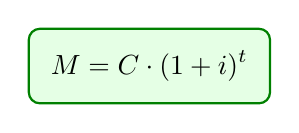
\begin{tikzpicture}
\node[rectangle, fill=green!10, rounded corners, inner sep=8pt, draw=green!50!black, thick] (box) {
$\displaystyle M = C \cdot (1 + i)^t$
};
\end{tikzpicture}
\vspace{0.5cm}

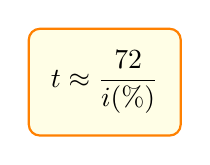
\begin{tikzpicture}
\node[rectangle, fill=yellow!10, rounded corners, inner sep=8pt, draw=orange, thick] (box) {
$\displaystyle t \approx \frac{72}{i(\%)}$
};
\end{tikzpicture}

\vspace{0.5cm}

\section*{Gabarito - Exercícios Básicos}

\begin{enumerate}[leftmargin=*]

\item \textbf{Calcule o montante a juros compostos:}

\begin{enumerate}[label=\alph*)]
\item $C = R\$ 1000$, $i = 2\%$ a.m., $t = 6$ meses

\textbf{\textcolor{blue}{Resolução}}
\[
M = C \cdot (1 + i)^t = 1000 \cdot (1 + 0,02)^6
\]
\[
M = 1000 \cdot (1,02)^6 = 1000 \cdot 1,126162 
\]
        \[ M \approx \resposta{1126,16} \]

\item $C = R\$ 500$, $i = 1,5\%$ a.m., $t = 12$ meses

\textbf{\textcolor{blue}{Resolução}}
\[
M = 500 \cdot (1 + 0,015)^{12} = 500 \cdot (1,015)^{12}
\]
\[
M = 500 \cdot 1,195618 \approx \resposta{R\$ 597,81}
\]

\item $C = R\$ 2000$, $i = 10\%$ a.a., $t = 2$ anos

\textbf{\textcolor{blue}{Resolução}}
\[
M = 2000 \cdot (1 + 0,10)^2 = 2000 \cdot (1,10)^2
\]
\[
M = 2000 \cdot 1,21 = \resposta{R\$ 2420,00}
\]
\end{enumerate}

\item \textbf{Calcule os juros compostos:}

\begin{enumerate}[label=\alph*)]
\item $C = R\$ 1500$, $i = 2\%$ a.m., $t = 8$ meses

\textbf{\textcolor{blue}{Resolução}}
\[
M = 1500 \cdot (1,02)^8 = 1500 \cdot 1,171659 = 1757,49
\]
\[
J = M - C = 1757,49 - 1500 = \resposta{R\$ 257,49}
\]

\item $C = R\$ 3000$, $i = 1\%$ a.m., $t = 1$ ano (12 meses)

\textbf{\textcolor{blue}{Resolução}}
\[
M = 3000 \cdot (1,01)^{12} = 3000 \cdot 1,126825 = 3380,48
\]
\[
J = 3380,48 - 3000 = \resposta{R\$ 380,48}
\]

\item $C = R\$ 5000$, $i = 12\%$ a.a., $t = 3$ anos

\textbf{\textcolor{blue}{Resolução}}
\[
M = 5000 \cdot (1,12)^3 = 5000 \cdot 1,404928 = 7024,64
\]
\[
J = 7024,64 - 5000 = \resposta{R\$ 2024,64}
\]
\end{enumerate}

\item \textbf{Complete a tabela:}

\begin{center}
\begin{tabular}{|c|c|c|c|}
\hline
\textbf{C} & \textbf{i} & \textbf{t} & \textbf{M (Compostos)} \\
\hline
R\$ 1000 & 2\% a.m. & 6 meses & \textcolor{blue}{R\$ 1126,16} \\
\hline
R\$ 500 & 12\% a.a. & 2 anos & \textcolor{blue}{R\$ 627,20} \\
\hline
R\$ 2000 & 1,5\% a.m. & 1 ano & \textcolor{blue}{R\$ 2390,00} \\
\hline
\end{tabular}
\end{center}

\textbf{Resolução da 2ª linha:}
\[
M = 500 \cdot (1,12)^2 = 500 \cdot 1,2544 = \resposta{R\$ 627,20}
\]

\textbf{Resolução da 3ª linha:}
\[
M = 2000 \cdot (1,015)^{12} = 2000 \cdot 1,195 = \resposta{R\$ 2390,00}
\]

\item \textbf{Problemas práticos:}

\begin{enumerate}[label=\alph*)]
\item Maria investiu R\$ 1500 a juros compostos de 2\% a.m. por 1 ano.

\textbf{\textcolor{blue}{Resolução}}
\[
M = 1500 \cdot (1,02)^{12} = 1500 \cdot 1,268242 = \resposta{R\$ 1902,36}
\]

\item Um capital de R\$ 2000 virou R\$ 2420 em 1 ano. Qual a taxa anual?

\textbf{\textcolor{blue}{Resolução}}
\[
2420 = 2000 \cdot (1 + i)^1 \Rightarrow 1 + i = \frac{2420}{2000} = 1,21
\]
\[
i = 0,21 = \resposta{21\%\ a.a.}
\]

\item Qual capital produz R\$ 3000 em 6 meses a 3\% a.m.?

\textbf{\textcolor{blue}{Resolução}}
\[
3000 = C \cdot (1,03)^6 \Rightarrow C = \frac{3000}{1,194052} \approx \resposta{R\$ 2512,58}
\]
\end{enumerate}
\end{enumerate}

\section*{Gabarito - Exercícios Intermediários}

\begin{enumerate}[leftmargin=*, start=5]

\item \textbf{Calcule as taxas equivalentes:}

\begin{enumerate}[label=\alph*)]
\item $2\%$ a.m. $\rightarrow$ taxa anual

\textbf{\textcolor{blue}{Resolução}}
\[
    (1,02)^{12} - 1 = 1,268242 - 1 = 0,268242 \]
\[\approx \resposta{26,82\%\ a.a.}\]

\item $12\%$ a.a. $\rightarrow$ taxa mensal

\textbf{\textcolor{blue}{Resolução}}
\[
    \sqrt[12]{1,12} - 1 = 1,009489 - 1 = 0,009489 \]
\[\approx \resposta{0,95\%\ a.m.} \]

\item $24\%$ a.a. $\rightarrow$ taxa mensal

\textbf{\textcolor{blue}{Resolução}}
\[
    \sqrt[12]{1,24} - 1 = 1,018087 - 1 = 0,018087 \] 
\[\approx \resposta{1,81\%\ a.m.} \]

\item $1\%$ a.m. $\rightarrow$ taxa anual

\textbf{\textcolor{blue}{Resolução}}
\[
    (1,01)^{12} - 1 = 1,126825 - 1 = 0,126825 \] 
\[\approx \resposta{12,68\%\ a.a.} \]
\end{enumerate}

\item \textbf{Um capital de R\$ 2000 foi aplicado a juros compostos:}

\begin{enumerate}[label=\alph*)]
\item Transformou-se em R\$ 2420 em 1 ano. Qual a taxa anual?

\textbf{\textcolor{blue}{Resolução}}
\[
2420 = 2000 \cdot (1 + i)^1 \Rightarrow 1 + i = 1,21 \Rightarrow \resposta{21\%\ a.a.}
\]

\item Virou R\$ 2650 em 8 meses. Qual a taxa mensal?

\textbf{\textcolor{blue}{Resolução}}
\[
2650 = 2000 \cdot (1 + i)^8 \Rightarrow (1 + i)^8 = 1,325
\]
\[
1 + i = 1,325^{1/8} = 1,0356 \Rightarrow \resposta{3,56\%\ a.m.}
\]

\item Qual o montante após 2 anos à taxa de 8\% a.a.?

\textbf{\textcolor{blue}{Resolução}}
\[
M = 2000 \cdot (1,08)^2 = 2000 \cdot 1,1664 = \resposta{R\$ 2332,80}
\]
\end{enumerate}

\item \textbf{Determine o tempo necessário:}

\begin{enumerate}[label=\alph*)]
\item Duplicar um capital a 10\% a.a. (use regra do 72)

\textbf{\textcolor{blue}{Resolução}}
\[
t \approx \frac{72}{10} = \resposta{7,2\ anos}
\]

\item Triplicar um capital a 5\% a.m.

\textbf{\textcolor{blue}{Resolução}}
\[
3 = (1,05)^t \Rightarrow t = \frac{\ln 3}{\ln 1,05} = \frac{1,098612}{0,048790} \]
\[ \approx \resposta{22,5\ meses} \]


\item R\$ 1000 virar R\$ 2000 a 2\% a.m.

\textbf{\textcolor{blue}{Resolução}}
\[
2 = (1,02)^t \Rightarrow t = \frac{\ln 2}{\ln 1,02} = \frac{0,693147}{0,019803} \approx \resposta{35\ meses}
\]
\end{enumerate}

\item \textbf{Problemas contextualizados:}

\begin{enumerate}[label=\alph*)]
\item Poupança: R\$ 5000 a 0,5\% a.m. por 2 anos (24 meses)

\textbf{\textcolor{blue}{Resolução}}
\[
M = 5000 \cdot (1,005)^{24} = 5000 \cdot 1,127159 = \resposta{R\$ 5635,80}
\]

\item CDB: R\$ 10000 a 12\% a.a. por 3 anos

\textbf{\textcolor{blue}{Resolução}}
\[
M = 10000 \cdot (1,12)^3 = 10000 \cdot 1,404928 = 14049,28
\]
\[
J = 14049,28 - 10000 = \resposta{R\$ 4049,28}
\]

\item Tesouro Direto: R\$ 8000 a 11,5\% a.a. por 5 anos

\textbf{\textcolor{blue}{Resolução}}
\[
M = 8000 \cdot (1,115)^5 = 8000 \cdot 1,723 = \resposta{R\$ 13784,00}
\]
\end{enumerate}
\end{enumerate}

\section*{Gabarito - Exercícios Avançados}

\begin{enumerate}[leftmargin=*, start=9]

\item \textbf{Análise de investimentos:}

\textbf{\textcolor{blue}{Resolução}}
\[
M_{CDB} = 10000 \cdot (1,12)^5 = 10000 \cdot 1,762342 = 17623,42
\]
\[
M_{Poupança} = 10000 \cdot (1,06)^5 = 10000 \cdot 1,338225 = 13382,25
\]
\[
\text{Diferença} = 17623,42 - 13382,25 = \resposta{R\$ 4241,17}
\]

\item \textbf{Tempo de aplicação com logaritmos:}

\begin{enumerate}[label=\alph*)]
\item Quanto tempo para R\$ 1000 virar R\$ 2000 a 5\% a.m.?

\textbf{\textcolor{blue}{Resolução}}
\[
2000 = 1000 \cdot (1,05)^t \Rightarrow 2 = (1,05)^t
\]
\[
t = \frac{\ln 2}{\ln 1,05} = \frac{0,693147}{0,048790} \approx \resposta{14,2\ meses}
\]

\item Se R\$ 5000 rendeu R\$ 1000 em 4 meses, qual a taxa mensal?

\textbf{\textcolor{blue}{Resolução}}
\[
6000 = 5000 \cdot (1 + i)^4 \Rightarrow (1 + i)^4 = 1,2
\]
\[
1 + i = 1,2^{1/4} = 1,046635 \Rightarrow \resposta{4,66\%\ a.m.}
\]

\item Em quanto tempo um capital quadruplica a 3\% a.m.?

\textbf{\textcolor{blue}{Resolução}}
\[
    4 = (1,03)^t \Rightarrow t = \frac{\ln 4}{\ln 1,03} = \frac{1,386294}{0,029559} \]
\[\approx \resposta{46,9\ meses}\]
\end{enumerate}

\item \textbf{Problema de lógica:}

\begin{enumerate}[label=\alph*)]
\item Um capital aplicado a juros compostos triplica em 5 anos. Em quanto tempo quadruplicaria?

\textbf{\textcolor{blue}{Resolução}}
\[
3 = (1 + i)^5 \Rightarrow 1 + i = 3^{1/5}
\]
\[
4 = (3^{1/5})^t = 3^{t/5} \Rightarrow \ln 4 = \frac{t}{5} \cdot \ln 3
\]
\[
    t = 5 \cdot \frac{\ln 4}{\ln 3} = 5 \cdot \frac{1,386294}{1,098612} = 5 \cdot 1,26186 \]
\[\approx \resposta{6,31\ anos} \]

\item Se a taxa é 2\% a.m., em quanto tempo o capital aumenta 50\%?

\textbf{\textcolor{blue}{Resolução}}
\[
    1,5 = (1,02)^t \Rightarrow t = \frac{\ln 1,5}{\ln 1,02} = \frac{0,405465}{0,019803} \] 
\[\approx \resposta{20,5\ meses} \]
\end{enumerate}

\item \textbf{Análise de gráfico:}

\begin{center}
\begin{tikzpicture}[scale=0.7]
\draw[->] (0,0) -- (6,0) node[right] {Meses};
\draw[->] (0,0) -- (0,5) node[above] {Montante (R\$)};
\draw[red, thick] (0,2) -- (1,2.1) -- (2,2.205) -- (3,2.315) -- (4,2.431) -- (5,2.553);
\foreach \x in {0,1,2,3,4,5} \draw (\x,0.1) -- (\x,-0.1) node[below] {\x};
\end{tikzpicture}
\end{center}

\begin{enumerate}[label=\alph*)]
\item Qual o capital inicial?

\textbf{\textcolor{blue}{Resolução}} No gráfico, quando $t = 0$, $M = 2000$. Portanto: \resposta{C = R\$ 2000}

\item Qual a taxa mensal aproximada?

\textbf{\textcolor{blue}{Resolução}} Em $t = 1$: $2100 = 2000 \cdot (1 + i) \Rightarrow 1 + i = 1,05 \Rightarrow \resposta{i = 5\%\ a.m.}$

\item Qual o montante após 10 meses?

\textbf{\textcolor{blue}{Resolução}}
\[
M = 2000 \cdot (1,05)^{10} = 2000 \cdot 1,62889 \approx \resposta{R\$ 3257,78}
\]
\end{enumerate}
\end{enumerate}

\end{multicols}

\end{document}
